
%!!! Theoretical stuff here with all needed formulas (examples are here too) !!!%

% macro for comfortable numerated formula create 
    \newcommand{\formula}[3]
    {
        \noindent#1\\[0.1cm]
        \begin{equation}\label{#2}
            #3
        \end{equation}
    }

% macro for in-text math formulas
    \newcommand{\mth}[1]
    {
        \begin{math}
            #1
        \end{math}
    }

% macro for Russian-named indexes in formulas
    \newcommand{\ruB}[1]
    {
        _{\text{#1}}
    }

\section{\Large Теоритическая часть }

\subsection{Формулы}

\noindentНаличие поверхностного слоя приводит к различию давлений по разные стороны от искривленной границы раздела двух сред.  Для сферического пузырька с воздухом  внутри жидкости избыточное давление задаётся формулой Лапласа:


\formula
{}
{Laplas}
{\Delta P = P\ruB{внутри} - P\ruB{снаружи} = \frac{2\sigma}{r}, }

\noindentгде \mth{\sigma} - коэффициент поверхностного натяжения, \mth{P\ruB{внутри} \text{\vspace{0.1cm} и \vspace{0.1cm}} P\ruB{снаружи}} - давление внутри пузырька и снаружи, r – радиус кривизны поверхности раздела двух фаз. Эта формула лежит в основе предлагаемого метода определения коэффициента поверхностного натяжения жидкости. Измеряется давление \mth{\Delta P} , необходимое для выталкивания в жидкость пузырька воздуха. \\[0.2cm]

\subsection{Схема установки}

Схема установки представлена на рисунке 1.

\begin{center}

    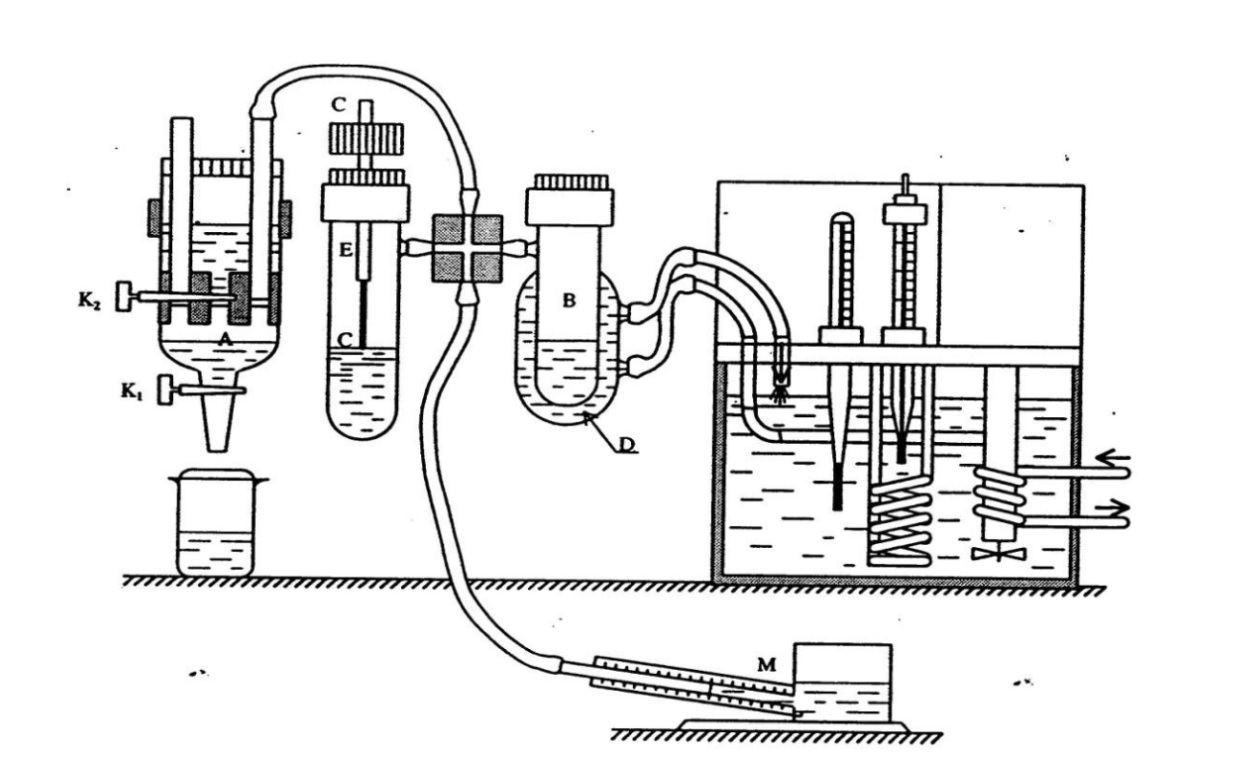
\includegraphics[scale=0.6]{picks/2_5_1_scheme1.jpg} \\
    \textit{\textcolor[HTML]{000000}{Рис. 1. Схема установки}}

\end{center}

\newpage